% Kapitel 1
% Die Unterkapitel können auch in separaten Dateien stehen,
% die dann mit dem \include-Befehl eingebunden werden.
%-------------------------------------------------------------------------------

\chapter{Einleitung}
%Hier Einleitungstext einfügen, dabei die Formatierungen selber erstellen
%Hier ist die Arbeitsweise des Systems anhand von State-Charts darzustellen und kurz zu erläutern.

Die Anwendung ist ein Werkzeug zur physikalischen Simulation und 3D-Visualisierung von Achterbahnfahrten.
Der Benutzer wählt dazu eine Datei mit der Spezifikation des Streckenverlaufes aus. Die Anwendung erstellt 
daraus ein virtuelles Modell der Achterbahn und simuliert physikalisch korrekt die Bewegung des Wagens mit
der Zeit. In den folgenden Abschnitten wird die Arbeitsweise des Simulators detailliert.

\section{Projektdetails}
Die Funktionalität der Anwendung gliedert sich in mehrere zusammenhängende Teilbereiche. Jeder dieser
Bereiche bündelt eine Reihe der Anforderungen, die im Pflichtenheft spezifiziert worden sind.

\subsection{Benutzeroberfläche}
Über die Benutzeroberfläche (GUI) werden dem Anwender alle vorhandenen Funktionen zugänglich gemacht.
Nach dem Programmstart befindet sich der Anwender in einem Initialzustand: Die Felder des 2D-Modells
und der 3D-Darstellung befinden sich in einem Blanko-Zustand und die physikalischen Parameter sind
auf die Standardwerte gesetzt. Der nächte Schritt ist die Auswahl einer Datei mit den Konstruktionsdaten
über ein Dateimenü. Nach dem Einlesen der Datei zeigt die Anwendung zunächst eine zweidimensionale 
Vorschau der Achterbahn an. Zu diesem Zeitpunkt können über ein Optionen-Menü verschiedene Anpassungen 
an den Grafikeinstellungen und den physikalischen Parametern vorgenommen werden. 
Aus der Vorschau heraus kann die Simulation gestartet werden. Ab diesem Zeitpunkt wird das Feld für 
die 3D-Darstellung befüllt. Auf Wunsch kann die 3D-Darstellung auf Bildschirmgröße
maximiert werden. Während der laufenden Simulation können die Grafikeinstellungen, nicht jedoch
die physikalischen Simulationsparameter angepasst werden. Wird die Simulation gestoppt, kehrt die Anwendung
wieder in die Vorschau zurück. Durch Schließen der Achterbahndatei gelangt der Benutzer wieder in den 
Initialzustand.

\begin{figure}
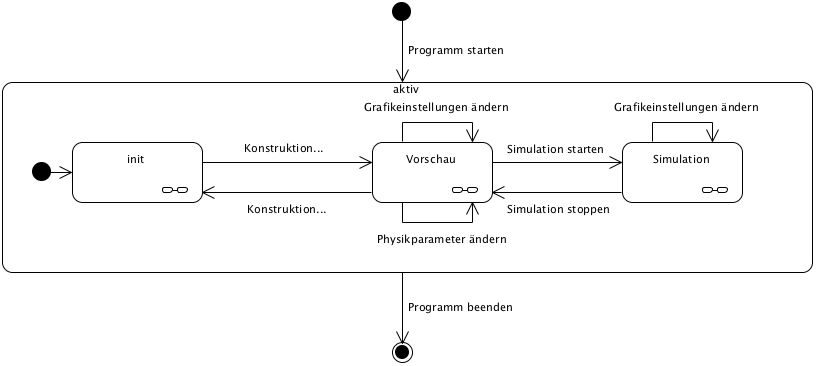
\includegraphics[width=\linewidth]{bilder/StateChart_GUI}
\caption{Statechart für die \textit{Benutzeroberfläche}}
\end{figure}

\subsection{Simulator}
Der Simulator ist das Kernstück der Anwendung und repräsentiert das Zusammenspiel aus physikalischen Berechnungen
und grafischer Darstellung der Achterbahnfahrt. Die Zustandswechsel des Simulators verlaufen synchron mit 
denen der Benutzeroberfläche. Nach dem Starten des Programms befindet sich der Simulator in einem Initialzustand,
der noch keine Simulation repräsentiert. Durch das Befüllen mit der Spezifikation der Achterbahn wird
eine Simulation instanziiert und zur Vorschau gebracht. Mit dem Start der Simulation werden in diskreten Zeitschritten
die aktualisierten physikalischen Daten eingelesen und zur Veränderung der Kameraposition verwendet. Durch das
Stoppen der Simulation kehrt auch der Simulator wieder in die Vorschau zurück.

\subsection{3D-Anzeige}
Die 3D-Anzeige dient zur Visualisierung der Achterbahnfahrt, also zur Darstellung der Bahn als 3D-Modell aus
einer vorgegebenen Kameraperspektive. Vor der Bereitstellung eines konkreten Achterbahnmodells befindet sich
die Anzeige in einem Initialzustand, in welchem es in Ermangelung von Daten nicht möglich ist, eine Szene darzustellen. 

\begin{figure}
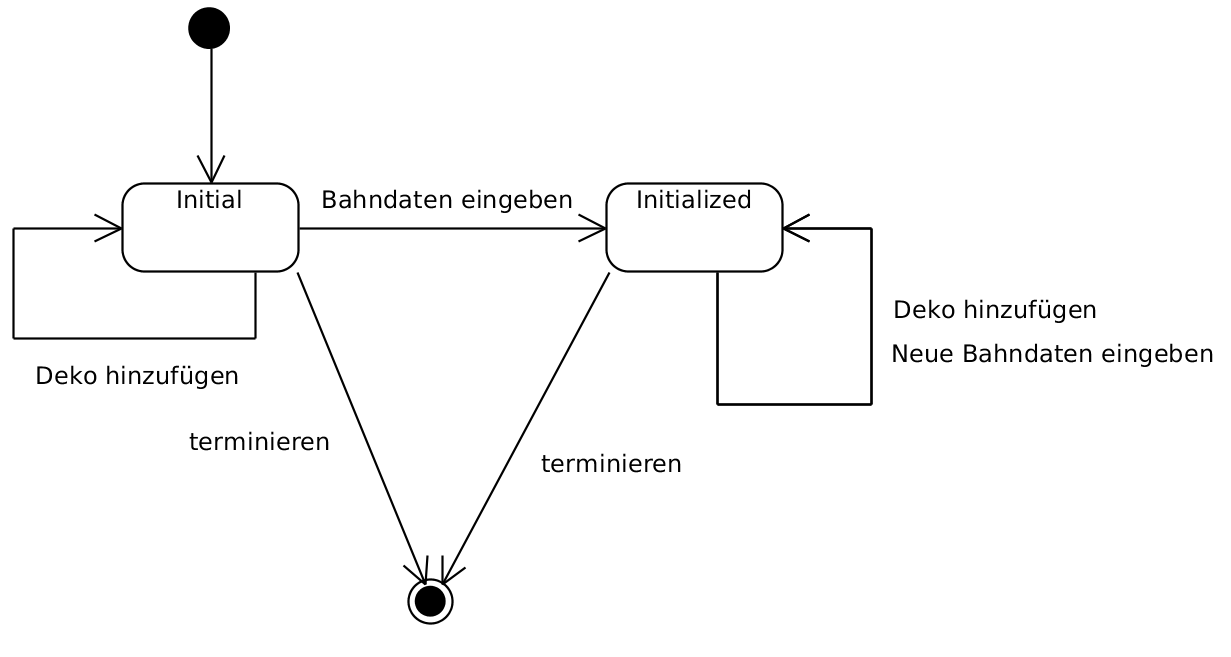
\includegraphics[width=\linewidth]{bilder/statechart_3dgraphics}
\caption{Statechart für die \textit{3D-Anzeige}}
\end{figure}

Durch Übergabe der Bahndaten kann die 3D-Anzeige die Achterbahn und deren Umgebung für die Anzeige vorberechnen.
Aber erst nach dem Start der Simulation, werden regelmäßig Bilder berechnet und angezeigt. Aus Sicht der 3D-Anzeige
können nach der Beladung jederzeit Änderungen wie Einfügen von Dekoration oder Anpassen der grafischen Einstellungen
vorgenommen werden, ohne das eine Zustandsänderung erforderlich wäre. Allerdings müssen innerhalb des Render-Vorgangs
eines einzelnen Bildes die Einstellungen unverändert bleiben, damit eine saubere Kommunikation mit dem 3D-Hardwarekontext
gewahrt bleibt.

\subsection{Physik und Mathematik}

Die physikalischen Berechnungen des Achterbahnsimulators folgen den Gesetzen der Newtonschen Mechanik für die Bewegung
eines Massenpunktes auf einer vorgegebenen Bahn im Gravitationsfeld der Erde. Berechnet wird die Bahnkurve als Lösung
einer gewöhnlichen Differentialgleichung mit vorgegebenen Anfangswerten. Die Lösung erfolgt nach einem numerischen
Verfahren, welches über die Zeit integriert.

Entsprechend wird der Zustand des Systems nach der Initialisierung mit den Bahndaten und den Anfangswerten von Zeitpunkt
zu Zeitpunkt weiterentwickelt, bis die Simulation (z.B. über Programmende) beendet wird.

Für die Berechnung der Bahnkurven kommen eine Reihe von Hilfsmethoden zum Einsatz. Diese Routinen sind zustandslos und
besitzen keinen eigenen Lebenszyklus.

\begin{figure}
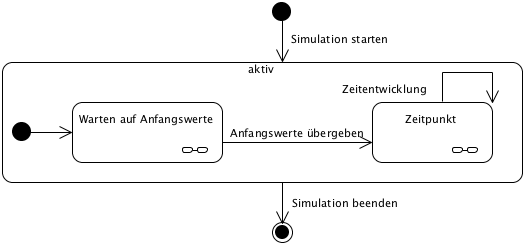
\includegraphics[width=\linewidth]{bilder/StateChart_physics}
\caption{Statechart für die \textit{Physik}}
\end{figure}
